%!TEX TS-program = pdflatex
\documentclass[b5paper,12pt,draft]{book}

\usepackage[utf8]{inputenc}
% \usepackage[T1]{fontenc}

\usepackage{charter}
\renewcommand{\rmdefault}{bch}

\usepackage{helvet}
\renewcommand{\sfdefault}{phv}

% \renewcommand{\familydefault}{\sfdefault} % \rmdefault

\usepackage[top=1.5cm, bottom=1.5cm, left=2.0cm, right=1.5cm]{geometry}
\setlength{\marginparwidth}{0.0pt}
\setlength{\footskip}{20.0pt}

% \usepackage{showframe} % DEBUG

\usepackage[final]{graphicx}

\usepackage{hyperref}
\hypersetup{final=true, colorlinks=true}
% \urlstyle{same}

\pagestyle {plain}


% Book
\begin{document}

% Title page
\begin{titlepage}
\vspace*{\stretch{2}}
\begin{center}
    \textbf{\huge{Croatian chess}} \\
    \large{and other variants} \\ [2.0cm]

    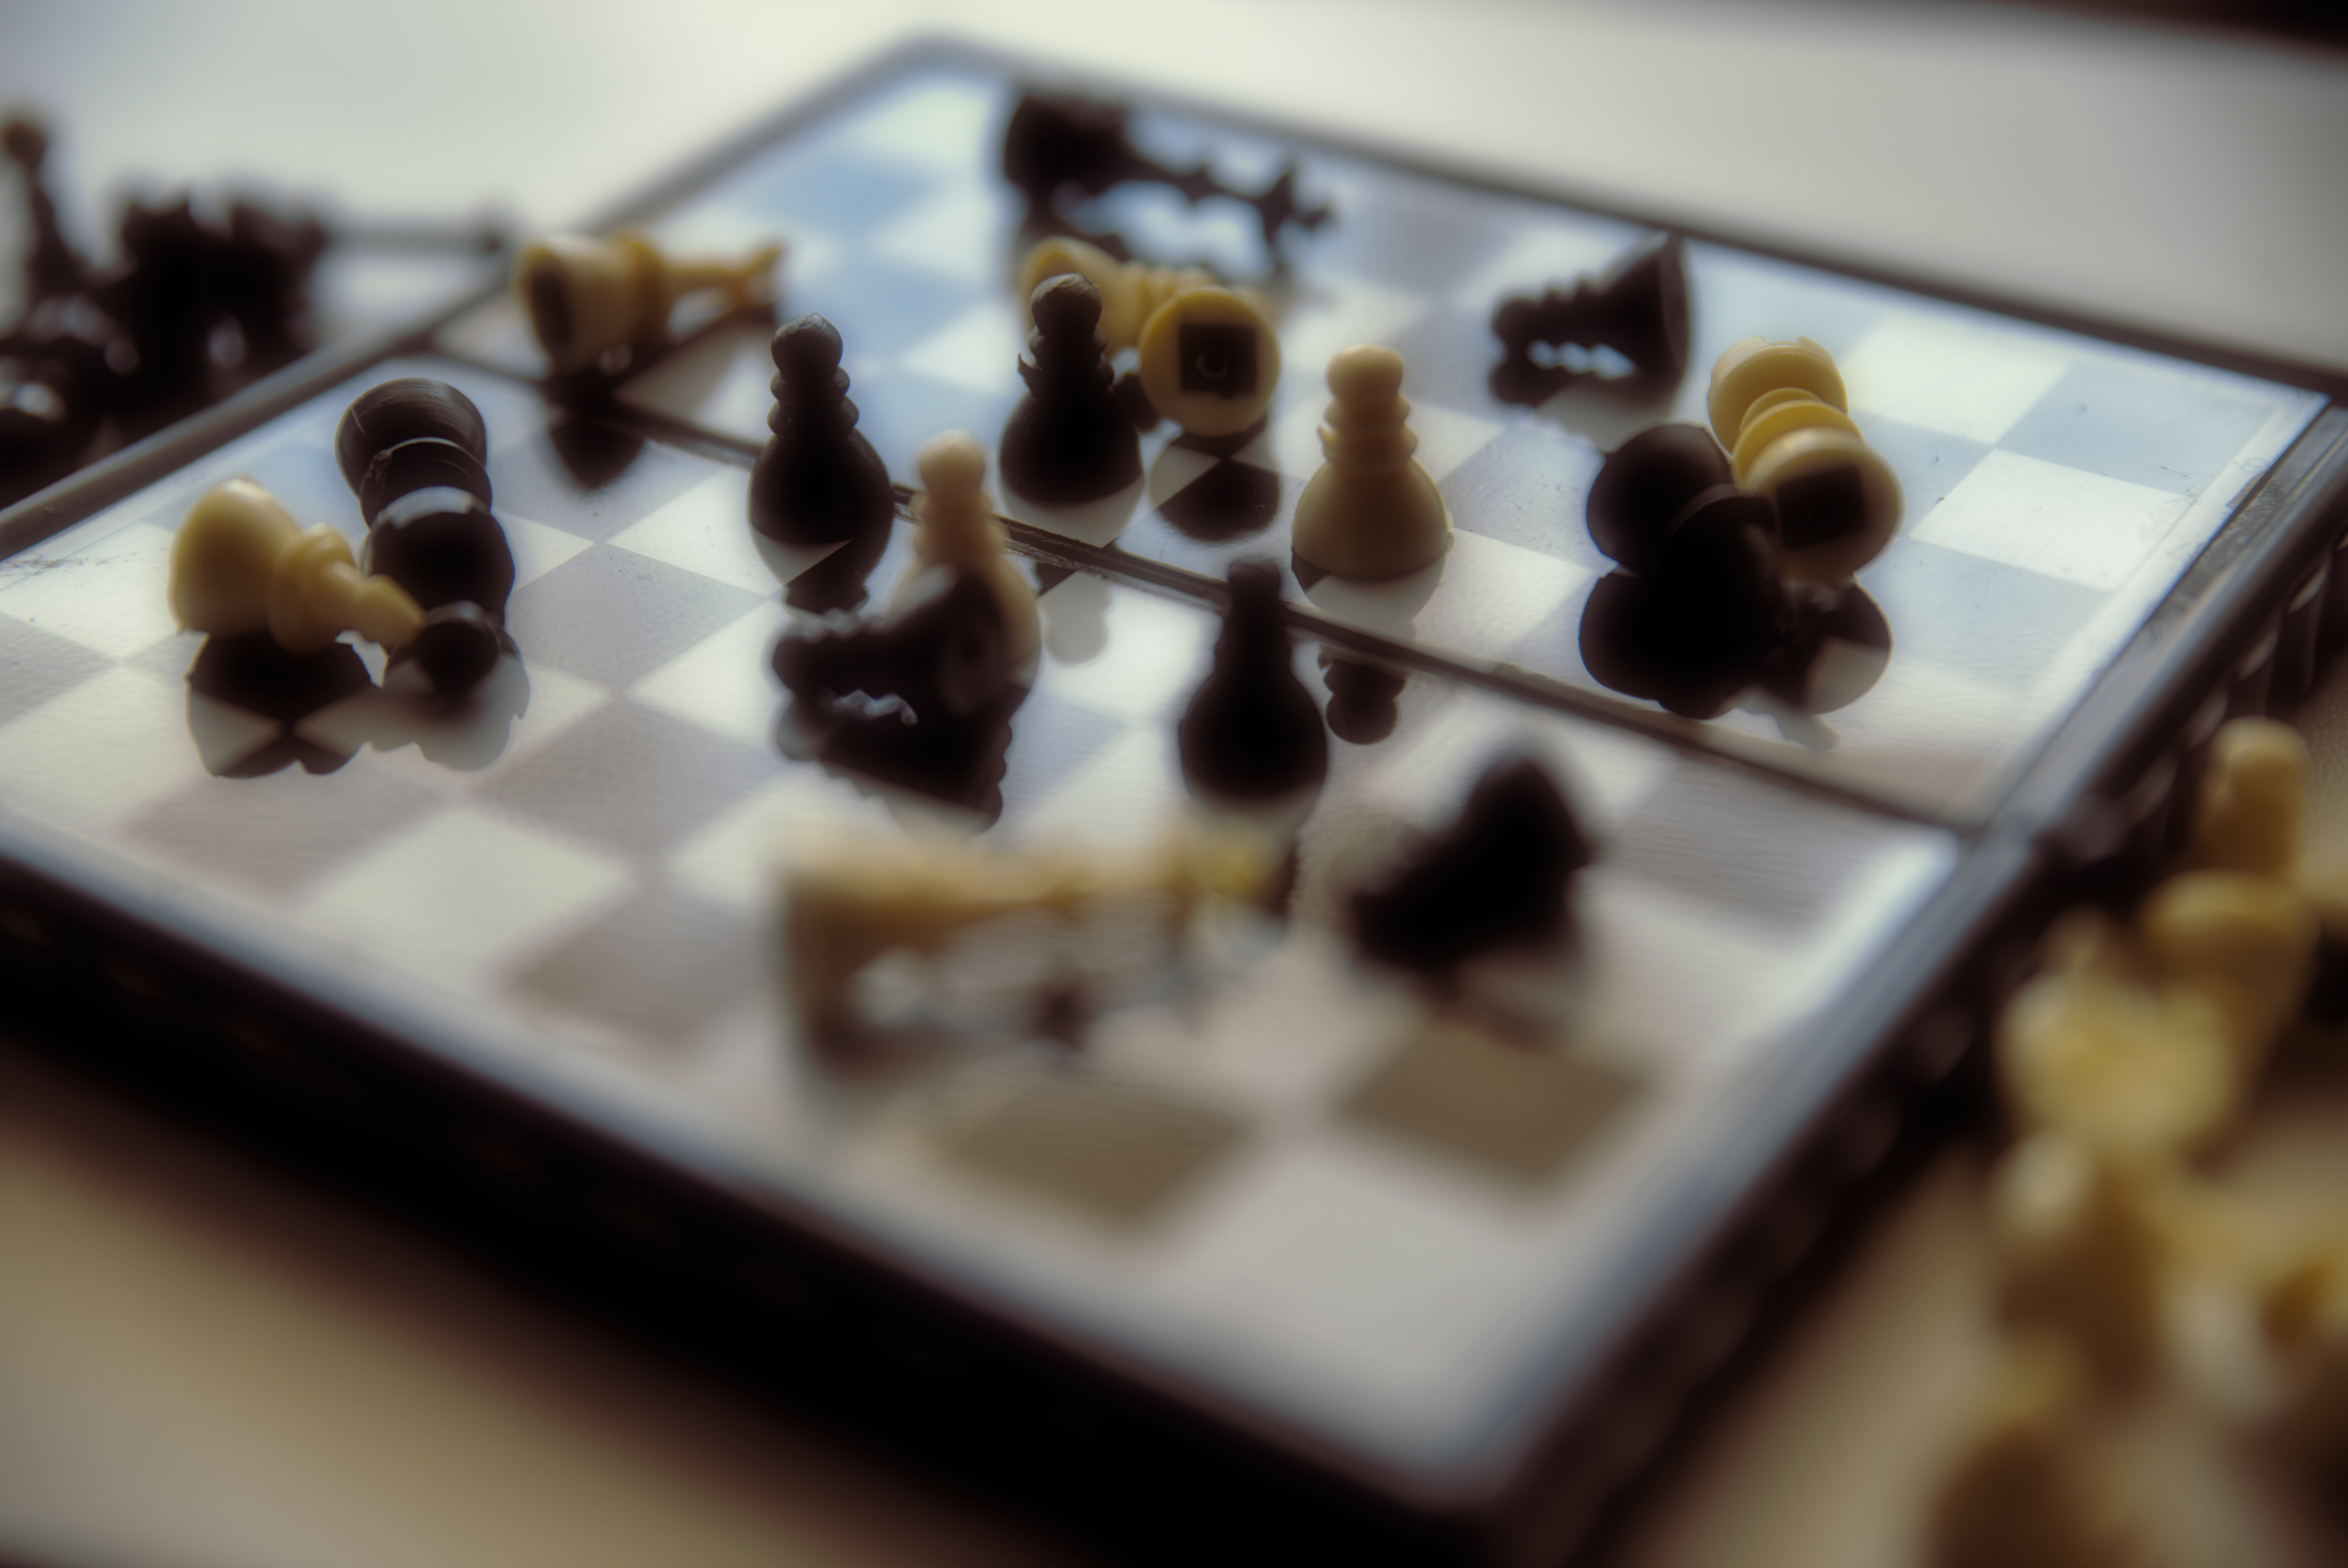
\includegraphics[width=0.9\textwidth, keepaspectratio=true]{../gfx/crochess.jpg} \\ [2.0cm]

    \textbf{\large{Mario Mlačak}} \\ [2.0cm]
\end{center}
\vspace{\stretch{1}}
\end{titlepage}

% Empty page
\thispagestyle{empty}
\vspace*{0.1\textheight}
\clearpage

% Dedication page
\thispagestyle{empty}
\vspace*{0.2\textheight}
\hfill{Dedicated to Miranda.}
\clearpage

% Publisher page
\thispagestyle{empty}
\vspace*{0.1\textheight}
\begin{center}
    \emph{Mario Mlačak} \\
    \textbf{Croatian chess} \\
    and other variants \\ [2.0em]

    \emph{Copyright} \\
    \copyright \hspace{0.2ex} 2009 -- 2016 Mario Mlačak \\
    \href{mailto:mmlacak@gmail.com}{mmlacak@gmail.com} \\ [2.0em]

    \emph{Legal} \\
    This book is published as Public Domain work. \\
    \href{https://en.wikipedia.org/wiki/Public\_domain}{https://en.wikipedia.org/wiki/Public\_domain} \\ [2.0em]

    \emph{Third, revised edition} \\
    \today \\
    Zagreb

    \vfill

    \LaTeXe
    \vspace{0.1\textheight}
\end{center}
\clearpage

% Inner title page
\thispagestyle{empty}
\vspace*{0.2\textheight}
\begin{center}
    \textbf{\Large{Croatian chess}} \\ [1.0em]
    \large{and other variants} \\ [1.0em]
    \small{3rd, revised edition} \\ [2.0cm]
    \vspace*{0.2\textheight}

    \textbf{\large{Mario Mlačak}} \\ [1.0em]
    \small{\today} % \\ [2.0cm]
\end{center}
\clearpage

% Empty page
\thispagestyle{empty}
\vspace*{0.1\textheight}
\clearpage

% Gratitude page
\thispagestyle{empty}
\vspace*{0.2\textheight}
\hfill{My most sincere gratitude to:}
\vspace*{1.0em}

\hfill{Valentina Štefanić} \\
\hspace*{\fill}{Kristina Mlačak} \\
\hspace*{\fill}{Slavko Štefanić}
\vspace*{1.0em}

\hfill{and many, many others.}
\vspace*{1.0em}

\hfill{Thank you all.}
\clearpage

% Empty page
\thispagestyle{empty}
\vspace*{0.1\textheight}
\clearpage

% Introduction page
\section{Introduction}
\small{This chapter's content... \\
abcdefghijklmnopqrstuvwxyz \\
ABCDEFGHIJKLMNOPQRSTUVWXYZ \\
0123456789}

\tiny{This chapter's content... \\
abcdefghijklmnopqrstuvwxyz \\
ABCDEFGHIJKLMNOPQRSTUVWXYZ \\
0123456789}

\normalsize{This chapter's content... \\
abcdefghijklmnopqrstuvwxyz \\
ABCDEFGHIJKLMNOPQRSTUVWXYZ \\
0123456789}

\section{Structure}
\small{This section's content... \\
abcdefghijklmnopqrstuvwxyz \\
ABCDEFGHIJKLMNOPQRSTUVWXYZ \\
0123456789}

\tiny{This section's content... \\
abcdefghijklmnopqrstuvwxyz \\
ABCDEFGHIJKLMNOPQRSTUVWXYZ \\
0123456789}

\normalsize{This section's content... \\
abcdefghijklmnopqrstuvwxyz \\
ABCDEFGHIJKLMNOPQRSTUVWXYZ \\
0123456789}

% Empty, enumerated page
\vspace*{0.1\textheight}
\clearpage

% List of figures
\listoffigures

% List of tables
\listoftables

% Table of contents
\tableofcontents
\clearpage

% % Empty page
% \thispagestyle{empty}
% \vspace*{0.1\textheight}
% \clearpage

% Challenge, end cover page
\thispagestyle{empty}
\begin{quotation}
    \it
    No FPS and racing sim [is a real challenge]. That is for
    dummies. This will make players of the game into new
    super-geniuses. Challenge to the max[imum] ... how much
    combinations there are in that [last variant] with
    teleportation, unicorn, pyramid, winged horse [Pegasus]
    and wave. How much more challenging it is compared to
    classic [chess]. Just Croatian [Ties] doubled number of
    possible combinations ...
\end{quotation}
\hspace*{\fill}{\textbf{Slavko Štefanić} [via e-mail]}
\vfill
\hspace*{\fill}{\LaTeXe}
\clearpage

\end{document}
